%%%%%%%%%%%%%%%%%%%%%%%%%%%%%%
\chapter{Background}

In this chapter, details regarding the simulation theory are gone over.  

%%%%%%%%%%%%%%%%%%%%%%%%%%%%%%
\section{Reactor Analysis}

reactors in general, LWR, fast breeders, GenIV, waste streams, power conversion

fission chain reaction, 7 factor formula?

coupling between TH, need for fast simulations in oder to do convergence iterations




%%%%%%%%%%%%%%%%%%%%%%%%%%%%%%
\subsection{History}

The Monte Carlo method is not a new way to simulate nuclear reactors (or any particle transport problem for that matter) and in it's modern form dates back to 1940 when XXX invented the approach while working on the Manhattan Project[cite]. Uncle in Monaco...  During this time, Henry Metropolis and John Von Neumann...[cite]  Although this may be disputed by some people since is was rumored that Enrico Fermi was basically doing small scale simulations of this kind in his head trying to get the Chicago Pile critical [cite].



%%%%%%%%%%%%%%%%%%%%%%%%%%%%%%
\subsection{Nuclear Interactions}

The core of a Monte Carlo simulation is explicitly modeling the individual interactions the neutron undergoes as it moves through matter.  At the highest level, these reactions can be broken down into two categories, elastic reactions and inelastic reactions.  Elastic reactions are those where both momentum and kinetic energy are conserved, i.e. ones where any energy the neutron loses is given to the target nucleus.  Inelastic reactions are those that conserve momentum but do not conserve kinetic energy, i.e. ones where the kinetic energy of the particles can be converted to a vibrational mode of the target nucleus, etc.  These reactions are further divided by the number and type of secondary particles they produce.  Reactions that produce no secondary neutrons are called ``disappearance'' reactions since the neutron effectively disappears, reactions that produce a single neutron are typically called scattering reactions since they effectively change the incoming neutron's energy and direction, and reaction the produce more than one particle are simply called ``secondary-producing'' reactions. Table \ref{nuc_reaction_summary} show a summary of the reaction classifications, and it can be seen that elastic scattering is the only elastic reaction.   

potential scattering vs compound nucleus.

\begin{table}[h]
\centering
\caption{Summary matrix of how neutron reactions are classified.}
\label{nuc_reaction_summary}
\begin{tabular}{| l | c | c | c |}
\multicolumn{4}{c}{Number of Secondaries} \\
\hline
  & 0 & 1 & $>$1 \\
 \hline
 Elastic & & Elastic Scatter & \\
 \hline
 Inelastic & Disappearance & Inelastic Scatter & Secondary-Producing \\
\hline
\end{tabular}
\end{table}

The probabilities for individual reactions occurring are expressed in terms of cross sections.  In simple terms, nuclear cross sections are like a geometric cross sections -they represent the ``size'' of the target nucleus for a particular reaction.  The classical analogy is that if neutrons and nuclei are hard spheres, and neutrons are randomly shot through a material, more neutrons will hit the larger targets than the smaller ones.  Cross sections are also expressed in units of area, the ``barn,'' which is $10^{-24}$ cm$^2$.  This unit was coined by Baker and Holloway while performing scattering experiments with uranium since ``a cross section of $10^{-24}$ cm$^2$ for nuclear purposes was really as big as a barn''\cite{LAMS523}.  Of course, nuclear cross sections have no literal meaning in terms of the actual sizes of the nuclei, they only represent the likelihood of a particular reaction occurring.  Working from the macroscopic scale, which is where measurements are taken, a \emph{macroscopic cross section}, represented by greek capital sigma ($\Sigma$), is the probability of a reaction happening within an infinitesimal distance d$x$.  With this parameter, we can write down an equation that describes the survival probability of a group of particles.  Describing a group is necessary since the dimension x is \emph{continuous}.  Given a particle packet containing N particles and $\Sigma$, their interaction probability over $d$x, the change the population over $d$x is the product of the population N and the interaction probability, as show in \eqref{pop_diff}.

\begin{equation}
\frac{d\mathrm{N}}{d\mathrm{x}} = - \Sigma \mathrm{N}
\label{pop_diff}
\end{equation}

Integrating \ref{pop_diff} over an interval yields an expression for the number of \emph{non-interacting} particles left in a packet after crossing that interval.  Dividing the surviving number by the initial gives a dimensionless expression for the non-interaction probability, P$_\mathrm{NI}$, over the interval x$_1$ as shown in \eqref{pop_NI}.

\begin{equation}
\mathrm{P}_\mathrm{NI} = \frac{\mathrm{N}}{\mathrm{N}_0} = \mathrm{e}^{- \Sigma \mathrm{x}_1}
\label{pop_NI}
\end{equation}

\begin{equation}
\Sigma = \frac{ - \mathrm{ln}(    \mathrm{I} / \mathrm{I}_0  )  }  {\mathrm{x}_1}
\label{pop_beam}
\end{equation}

Since these expressions also apply to beam intensity, they can be used to measure the cross sections for materials by rearranging the equations into the form shown in \eqref{pop_beam}.  If the source intensity, the exiting intensity, and the material thickness are all known, the macroscopic cross section for that material can be determined.  On a microscopic level, however, the neutron interaction probabilities only depend on the type of nucleus, not the aggregate material.  To correct for this, the measured macroscopic cross section can be divided by the number density of nuclei in the material to give the microscopic cross section, $\sigma$, which is material-independent and only depends on the isotope.  In \eqref{micro_exp}, N represents the number density in units of cm$^{-3}$, $\rho$ represents the material density in terms of g*cm$^{-3}$, and M represents the nuclear mass in g.  The microscopic cross section has units of barns, and is what is given in nuclear data files.  They are more general since they are not material-dependent and can be summed into a total material macroscopic cross section by weighting individual microscopic cross sections with the number density of an isotope in a material, as show in \eqref{material_sum_xs}.  In this expression, $f_\mathrm{i}$ is the atomic fraction of isotope i in the material.


\begin{equation}
\Sigma = N \sigma = \frac{\rho}{M} \sigma
\label{micro_exp}
\end{equation}

\begin{equation}
\sum_{\mathrm{i}=1}^{\mathrm{N}_\mathrm{isotopes}} f_\mathrm{i} =1
\label{fraction_norm}
\end{equation}

\begin{equation}
\Sigma_{\mathrm{material}} = \mathrm{N}_1 \sigma_1 +  \mathrm{N}_2 \sigma_2 + \mathrm{N}_3 \sigma_3+ ... = \sum_{\mathrm{i}=1}^{\mathrm{N}_\mathrm{isotopes}} \mathrm{N}_\mathrm{i} \sigma_\mathrm{i} = \rho\frac{\sum_{\mathrm{i}=1}^{\mathrm{N}_\mathrm{isotopes}} f_\mathrm{i}\sigma_\mathrm{i} } { \sum_{\mathrm{i}=1}^{\mathrm{N}_\mathrm{isotopes}} f_\mathrm{i} \mathrm{M}_\mathrm{i}}
\label{material_sum_xs}
\end{equation}

The above expressions do not take energy into account, so they are assumed to be at a single energy.  Using such simple expressions to determine the cross section of an isotope would only be valid with the use of a very, very precisely mono-energetic beam.  The quantum mechanical details that go into cross sections can cause them to depend strongly on the energy (or velocity) of the neutron and the target nucleus.  Many nuclides have resonances where the interactions probability spikes to very large values.  This typically happens when the incoming energy is exactly that of an energy level of the resultant compound nucleus \cite{duderstadt}.   Figure \ref{xs_e_dependence_li} shows the energy dependence of various reactions type in lithium-6 and Figure \ref{xs_e_dependence_u} shows the dependence of others in uranium-235.  

\begin{figure}[h!]
  \label{xs_e_dependence_li}
  \centering
    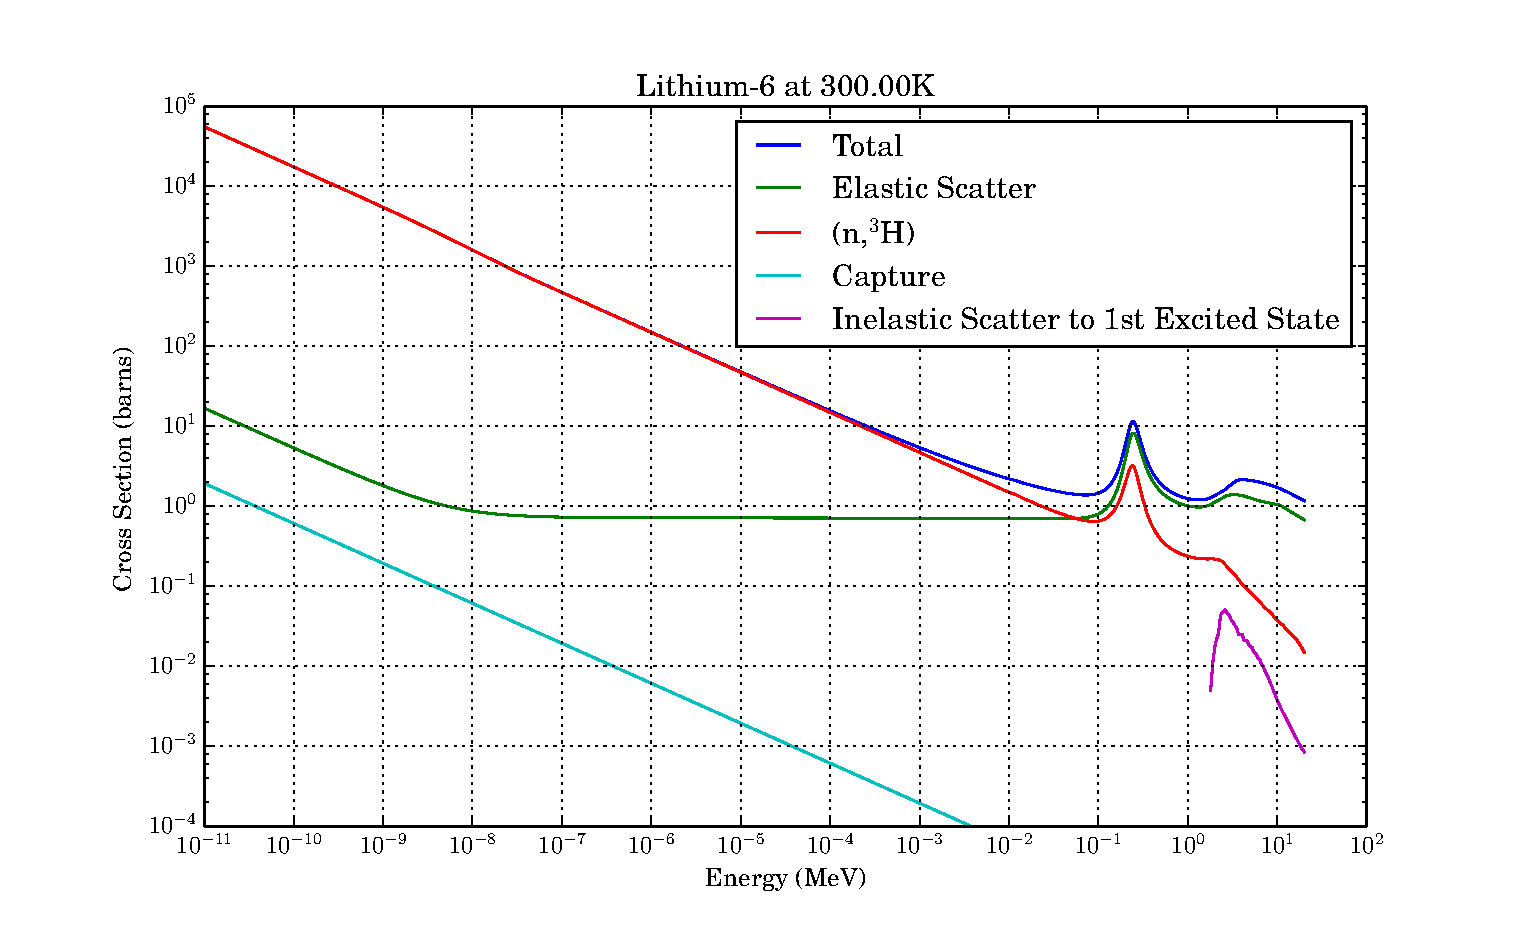
\includegraphics[width=0.8\textwidth]{graphics/xs_li6.eps}
     \caption{The energy dependence of some reactions in lithium-6.}
\end{figure}

\begin{figure}[h!]
  \label{xs_e_dependence_u}
  \centering
    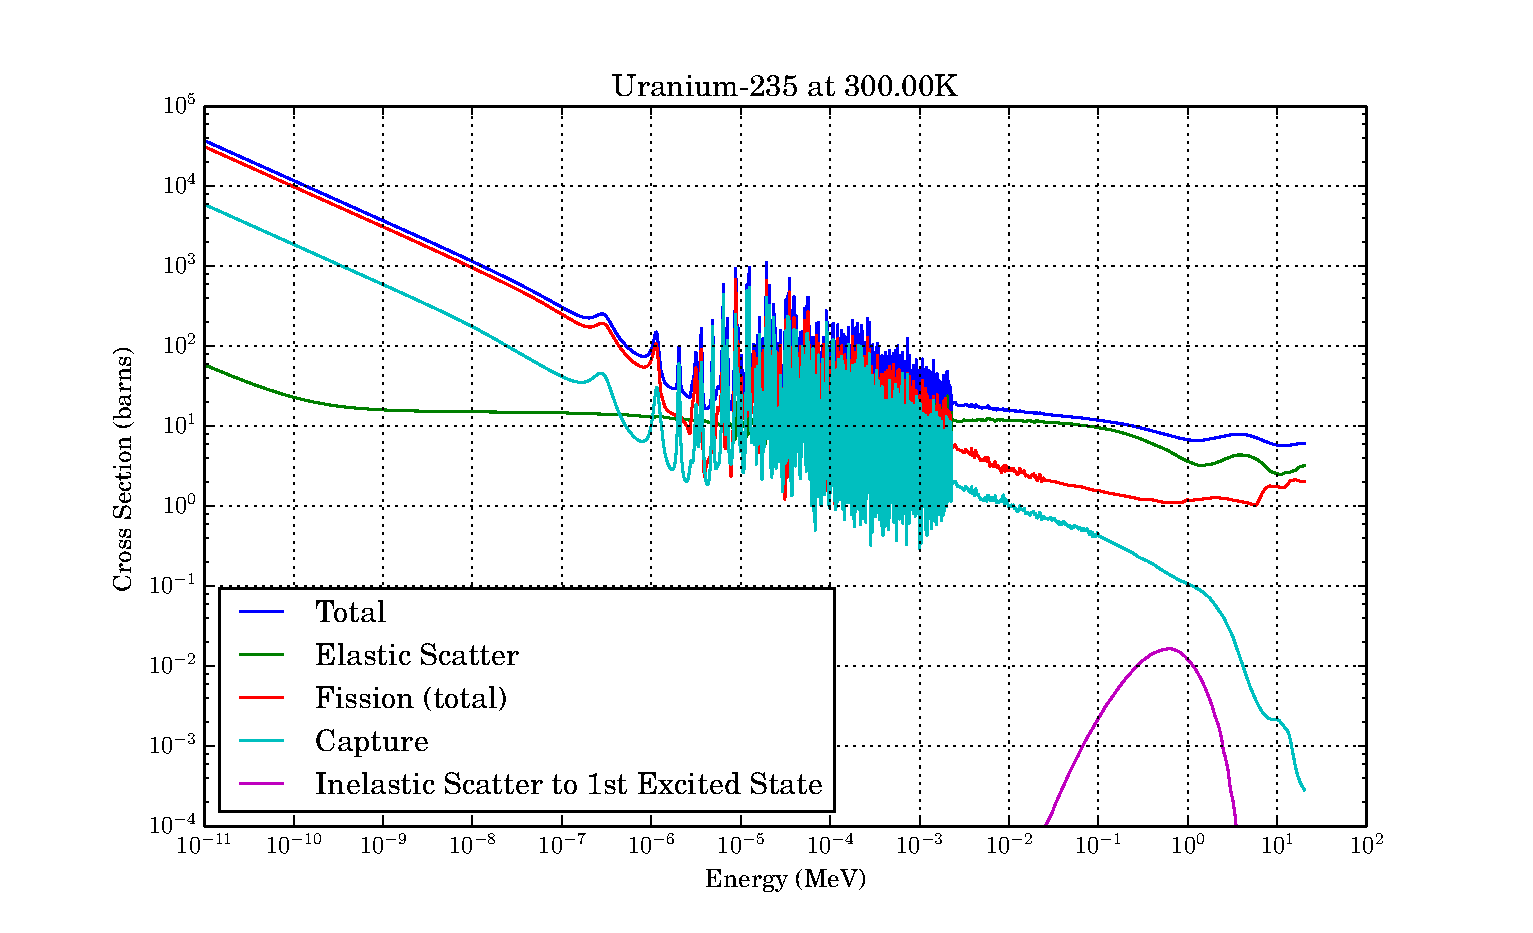
\includegraphics[width=0.8\textwidth]{graphics/xs_u235.eps}
    \caption{The energy dependence of some reactions in uranium-235.}
\end{figure}

It is important to note the complexity shown in uranium-235 in the 0.1eV to 40keV range.  This is referred to as the ``resonance region'' and adds much of the complexity in accurately modeling neutron transport.  There are no simple functional representations available for these types of cross sections, so they must be represented in a point-wise tabular format.  It is also important to note that at low energies, cross sections typically lose structure and exhibit the same ``1/$v$'' scaling.  This is due to the particle and the target having more time to interact with each other.  The energy levels where this phenomenon exists is similar the thermal energy of the target and the target no longer appears stationary from the neutrons perspective.  If the neutron is slow enough, the targets appear to be moving instead of the neutron, and more of them come into the neutrons sphere of interaction.  This is the qualitative reason for 1/$v$ scaling at low energies.  Due to to their identical scaling, the ratios between the reaction types stays constant as velocity is decreased but the overall interaction probability with respect to distance increases.

In the next subsections, the characteristics and kinematics of the different reaction types are explained.

\subsubsection{Elastic Scattering}

Elastic scattering conserves both the momentum and the kinetic energy of the reacting particles and occurs when the neutron does not enter the nucleus, only bounces off of it's potential field.  Since there is only a single exiting particle, elastic scattering is a two-body interaction and the exiting energies can be determined if the angle between the exiting particle is known.  This problem is greatly simplified if the interacting particles' velocities are transformed into the center-of-mass (CM) frame, where net momentum is zero. The velocity of the CM is defined in \eqref{vCM} where $m$ and $M$ are the neutron's and the target's respective masses, $v$ and $V$ are their respective velocity vectors, and $A$ is the ratio of the target's mass to the neutron's mass (also know as the ``atomic weight ratio'' or AWR).  The derivation from here follows closely with that in ref \cite{jaakko}.

\begin{equation}
A = \frac{M}{m}
\label{AWR}
\end{equation}

\begin{equation}
\boldsymbol{v_{\mathrm{CM}}} = \frac{ m \boldsymbol{v} + M \boldsymbol{V} }    {m+M} = \frac{ \boldsymbol{v} + A \boldsymbol{V} }    {1+A}
\label{vCM}
\end{equation}

The CM velocities of the target and the neutron are then calculated by subtracting the CM velocity out of them, ash shown in \eqref{CM}.  The $_\mathrm{c}$ subscript will denote the CM-frame values from now on, whereas $v_{\mathrm{CM}}$ will denote the velocity of the CM frame relative to the lab frame.

\begin{equation}
\begin{split}
 \boldsymbol{v_{_\mathrm{c}}} &= \boldsymbol{v} - \boldsymbol{v_{\mathrm{CM}}} \\  
 \boldsymbol{V_{\mathrm{c}}} &= \boldsymbol{V} - \boldsymbol{v_{\mathrm{CM}}}
 \end{split}
\label{CM}
\end{equation}

Once in the CM frame, the equation for conservation of momentum can be written as \eqref{consMomCM}.  The primed values are those after the collision.  Since the net momentum is zero, the directions of the neutron and the target must be in opposite directions as shown in \eqref{rotationCM}.

\begin{equation}
\begin{split}
m \boldsymbol{v_{_\mathrm{c}}} + M \boldsymbol{V_{_\mathrm{c}}} &= m \boldsymbol{v_{_\mathrm{c}}^\prime} + M \boldsymbol{V_{_\mathrm{c}}^\prime} = 0\\
    \boldsymbol{v_{_\mathrm{c}}} + A  \boldsymbol{V_{_\mathrm{c}}} &=     \boldsymbol{v_{_\mathrm{c}}^\prime} + A  \boldsymbol{V_{_\mathrm{c}}^\prime} = 0
\end{split}
\label{consMomCM}
\end{equation}

\begin{equation}
\begin{split}
\boldsymbol{v_{_\mathrm{c}}^\prime} &= - A  \boldsymbol{V_{_\mathrm{c}}^\prime} \\
\boldsymbol{v_{_\mathrm{c}}} &= -A  \boldsymbol{V_{_\mathrm{c}}}
\end{split}
\label{rotationCM}
\end{equation}

The equation for conservation of energy is shown in \ref{consECM}.  Energy is a scalar quantity, and therefore these equations are as well.  There are no vectors, which are indicated with boldface type, since $v^2 =( \boldsymbol{v} \cdot \boldsymbol{v})$.  $Q$ is the amount of energy released by the reaction, and is zero here but is convenient to include in this derivation for use in inelastic collision kinematics where it is nonzero.

\begin{equation}
\begin{split}
m v_{_\mathrm{c}}^2 + M V_{_\mathrm{c}}^2 &= m v_{_\mathrm{c}}^{\prime2} + M V_{_\mathrm{c}}^{\prime2} + 2Q \\
    v_{_\mathrm{c}}^2 + A  V_{_\mathrm{c}}^2 &=     v_{_\mathrm{c}}^{\prime2} + A  V_{_\mathrm{c}}^{\prime2} + \frac{2Q}{m}
\end{split}
\label{consECM}
\end{equation}

There are now two unknowns (the primed values) and two equations, and the final velocities of the neutron and the target can be determined.  Substituting \eqref{rotationCM} into \eqref{consECM} and solving yields either equation in \eqref{finalvCM}, depending on how the substitution is done.  It can be seen that if $Q$ is zero, as it is in elastic scattering, the initial and final velocities are the same for the particles and the interaction only causes a rotation in the CM frame.

\begin{equation}
\begin{split}
v_{_\mathrm{c}}^{\prime} &=  \sqrt{ v_{_\mathrm{c}}^{2} + \frac{2AQ}{m(A+1)}  }  \\
V_{_\mathrm{c}}^{\prime} &= \sqrt{ V_{_\mathrm{c}}^{2} + \frac{2Q}{mA(A+1)}  } 
\end{split}
\label{finalvCM}
\end{equation}

At first glance, it seems like the interaction has been fully characterized, but \eqref{rotationCM} only relates the initial states of the neutron and the target to one another and the final states of neutron and the target to one another.  The initial state and final state of the neutron still need to be related.  It has been mentioned already that the interaction is only a rotation in the CM frame, so the initial and final state of the neutron's direction can be related by a three-dimensional rotation formula.  An efficient algorithm is given by the Rodrigues' rotation formula, shown in \eqref{RodriguesRot}.  In the formula, $\boldsymbol{k}$ is an auxilliary unit vector around which $\boldsymbol{v}$ is being rotated.  From this unit vector, $theta$ is the angle $\boldsymbol{v}$ is rotated away from $\boldsymbol{k}$ such that $(\boldsymbol{v} \cdot \boldsymbol{v_{\mathrm{rot}}}) = |v||v_{\mathrm{rot}}|\cos\theta$.  It is ``efficient'' in the sense that to rotate a vector, a full 3x3 matrix does not need to be constructed and multiplied by the vector. In other words, matrix-vector operations are not needed and it can be carried out with only vector operations \cite{}.

\begin{equation}
 \boldsymbol{ v_{ \mathrm{rot}}} = \boldsymbol{v} \cos \theta + (\boldsymbol{k} \times \boldsymbol{v}) \sin \theta + \boldsymbol{k} (\boldsymbol{k} \cdot \boldsymbol{v})(1-\cos \theta)
\label{RodriguesRot}
\end{equation}

If the polar and azimuthal rotation angles, $\theta$ and $\phi$, respectively, are determined, the initial neutron velocity vector can be rotated through these angles to its final value.  After the rotation is done, the final velocities are known in the CM frame and they can be transformed back to the lab frame to give the final velocities there, as shown in \eqref{xformbackCM}.

\begin{equation}
\begin{split}
 \boldsymbol{v^{\prime}}  &= \boldsymbol{v_{\mathrm{c}}^{\prime}} + \boldsymbol{v_{\mathrm{CM}}} \\  
 \boldsymbol{V^{\prime}} &= \boldsymbol{V_{\mathrm{c}}^{\prime}} + \boldsymbol{v_{\mathrm{CM}}}
 \end{split}
\label{xformbackCM}
\end{equation}


\subsubsection{Inelastic Level Scattering}

Inelastic scattering is the other type of scattering a neutron can undergo where kinetic energy is no longer conserved.  An amount of energy is either released from the reaction to the particles, or more commonly, taken from the particles and lost to the reaction.  In neutron-nucleus collisions, the target nucleus can be excited to a higher energy state than its ground state if the colliding neutron has a high enough energy to do so.  If it does and the collision excites the nucleus, a discrete amount of energy equal to the energy of the excited state is lost to the reaction.  These excited states typically do not have long half lives, and a gamma ray is emitted when the nucleus relaxes to its ground state.  This type of reaction is called inelastic level scattering due to a an excited energy \emph{level} becoming occupied by the target nucleus.  

Since it is still a two-body interaction, the kinematics of the reaction are identical to elastic scattering except the $Q$ value is nonzero and negative.  These reactions have a threshold energy below which their cross sections are zero since the neutron would not have enough energy to excite the state.   Figure \ref{Elevels} shows the energy levels in lead-XXX, which is often used as a fast neutron moderators due to its many, low-lying energy levels and its large inelastic scattering cross sections.

\begin{figure}[h!]
  \label{Elevels}
  \centering
    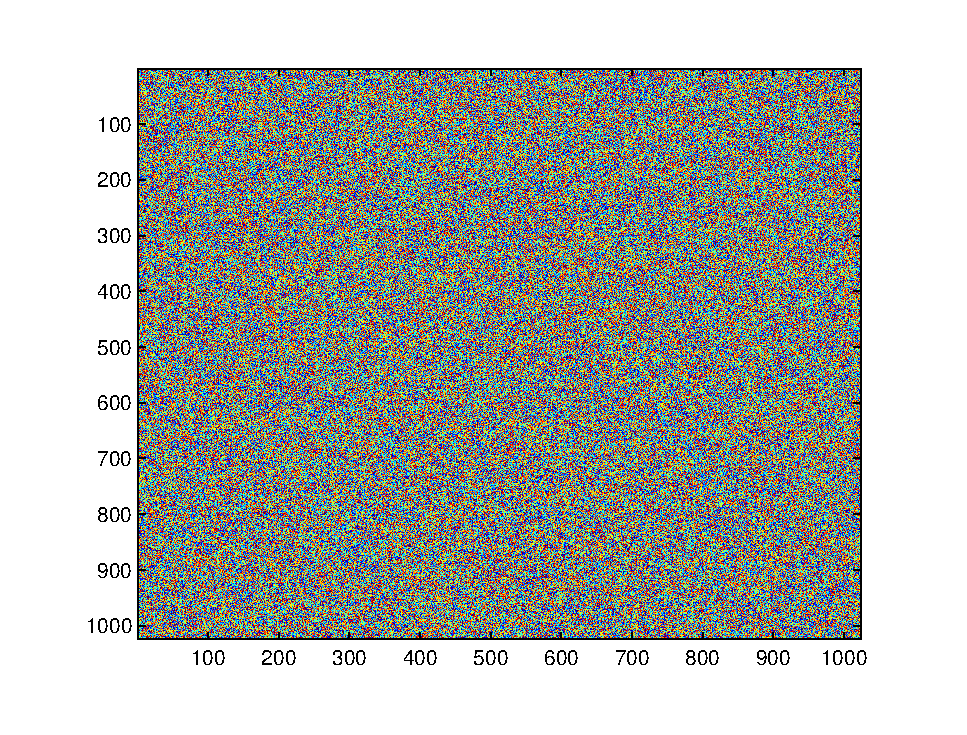
\includegraphics[width=0.8\textwidth]{graphics/noise.eps}
     \caption{The energy levels of lead-XXX\cite{}.}
\end{figure}

\subsubsection{Inelastic Continuum Scattering}

At energies above the distinct levels there lies a continuum in the nuclear energy states.  This isn't truly a ``continuum'' in the strictest sense, but the energy levels become so close together they they effectively form a domain where energy can take continuous values.  Unlike the discrete $Q$ values corresponding to a single excited state used in inelastic level scattering, the $Q$ value of the reaction now follows a distribution.  

In bound nuclei, S(a,b)

\subsubsection{Disappearance Reactions}

Unlike scattering reactions, where the energy and direction of the neutron is changed but continues to transport, \emph{disappearance} reactions remove a free neutron.  Typically this \emph{capture} of a neutron leaves the daughter nucleus in an excited state, which them relaxes to ground state by emitting a gamma ray.


\subsubsection{Fission}

Fission means ``the splitting splitting of something into two parts'' in the literal sense of the word.  This is exactly what nuclear fission is as well.  It is when a nucleus splits into two smaller nuclei, called \emph{fission fragments}.  When heavy nuclei undergo fission, they release energy, and typically emit a few other particles, including neutrons.  That this reaction releases energy is the reason heavy elements, like uranium, can be used as an energy source.  This is because the fission fragments have a higher binding energy per nucleon compared to the parent nucleus.  Figure \ref{binding_e_per_nuc} shows the average binding energy per nucleon for a wide range of isotopes.  Note that the peak of the curve is at Iron-56, the most tightly bound nucleus, and that heavier nuclides are lower than it.  Fission splits the parent into two lighter nuclides, and since the fragments are more tightly bound, the excess binding energy from the parent is released.  The released energy isn't simply deposited as heat directly, however, it is released in a range of forms.  Fission doesn't just release some energy, it releases a substantial amount of it.  Uranium-235, for example, releases a total of 192.9$\pm$0.5 \emph{MeV} per fission \cite{duderstadt}.  Compared to chemical energy sources where the energy released per reaction is on the order of 1\emph{eV}.  Fission energy yield is 8 orders of magnitude larger!  Not all of this energy is converted to heat, bit a substantial amount is.  Table \ref{fission_dist} shows the fraction of this total energy that is given to each entity.  Note that a significant fraction is given to neutrinos, which is essentially lost due to their very small interaction cross section.  The kinetic energy of the fission fragments has the majority of the energy, and since they are heavy and charged, their energy is deposited as heat very near to the fission site.  Other particles, light photons and neutrons, carry some of the fission energy further away from the fission site, but their energy mostly still ends up as heat.
  
\begin{figure}[h!]
\label{binding_e_per_nuc}
  \centering
    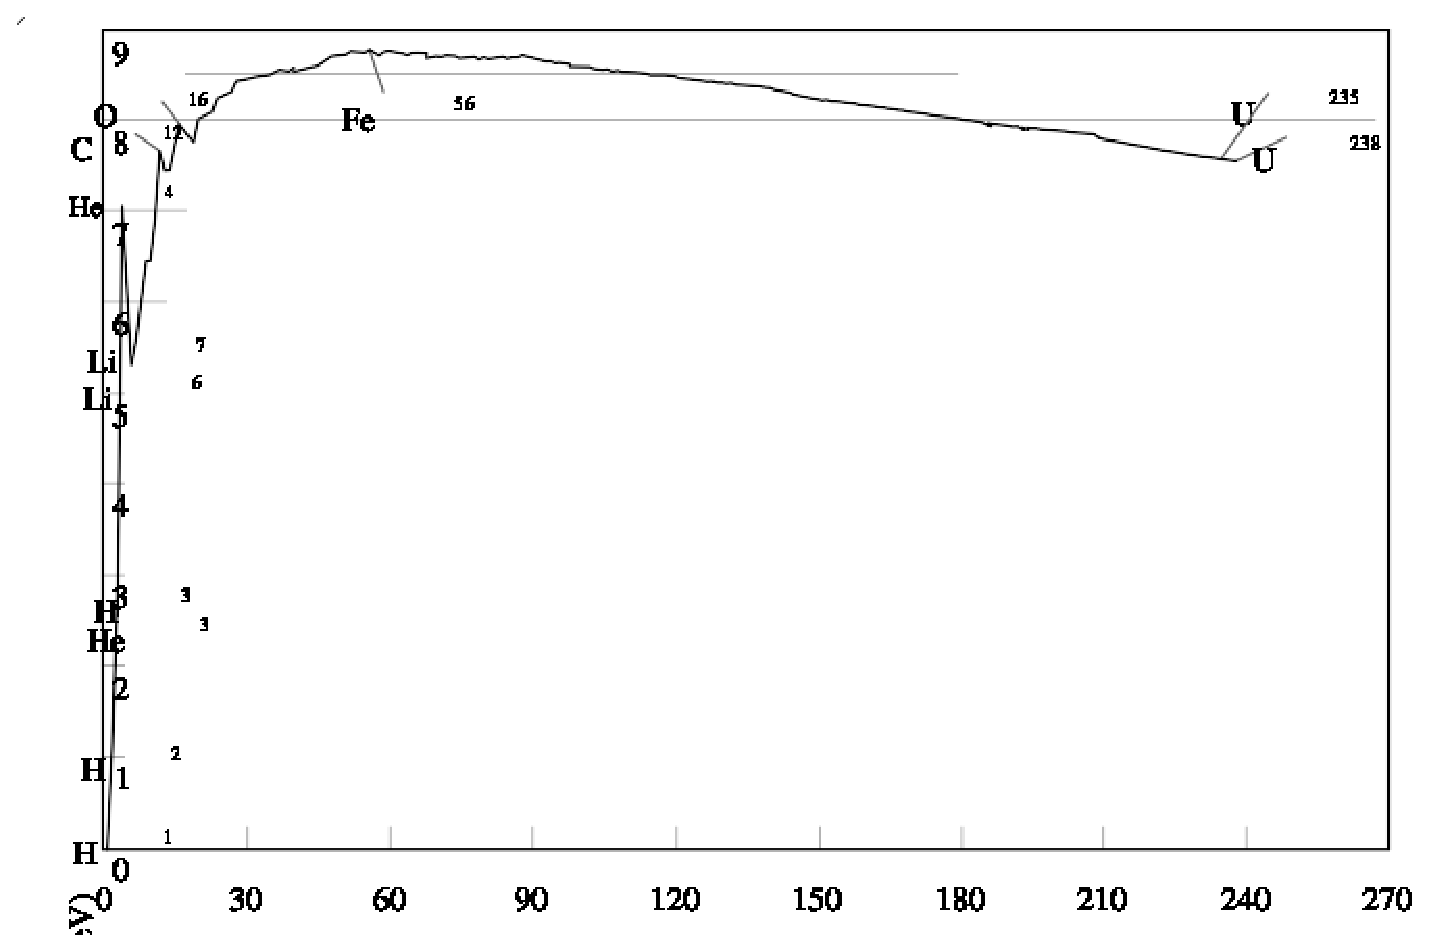
\includegraphics[width=0.8\textwidth]{graphics/binding_e_per_nuc.eps}
     \caption{Average binding energy per nucleon.  REPLACE ME WITH ONE YOU MAKE YOURSELF FROM DATA. \cite{}.}
\end{figure}

\begin{table}[h]
\centering
\caption{Average distribution of fission energy \cite{duderstadt}.}
\label{fission_dist}
\begin{tabular}{| l | c | r | r |}
\hline
Particle & Energy (\%) & Range & Time \\
\hline
Fission fragment kinetic energy & 80 & $<$0.1cm & prompt \\
\hline
Prompt neutrons & 3 & 10-100cm & prompt \\
\hline
Photons & 4 & 100cm & prompt \\
\hline
Fission product $\beta$ decay & 4 & short & delayed \\
\hline
Neutrinos &  5 & extremely long & delayed \\
\hline
Nonfission reactions from n capture & 4 & 100cm & delayed \\
\hline
\end{tabular}
\end{table}

Fission is technically considered a disappearance reaction as well since the fission-inducing neutron is absorbed by the nuclide.  Even though is is absorbed, more than 2 new neutrons are released by fission, enabling the fission chain reaction to occur.  An important parameter of the fission chain reaction is $nu$, the fission neutron yield.    The total yield is different than the prompt yield in that it also includes neutrons produced from photon-induced emission and from fission product decay.  These neutrons are not ``prompt'' in that they are not emitted immediately from the fission itself.  The processes that create these ``delayed'' neutrons (decay and nuclear relaxation) take time to occur.  Prompt neutrons appear immediately after fission, whereas delayed neutrons can appear anywhere between 0.6 to 80 seconds after.  The kinetics of a nuclear chain reaction depend heavily on the fraction the delayed neutrons which sustain the chain reaction.  Since they have a relatively large time delay, they cause the time between subsequent neutron generations to become longer.  This time between generations is called the \emph{effective neutron lifetime}, and is approximately $10^{-4}$ seconds for prompt neutrons and $0.1$ seconds for delayed neutrons in light water (thermal spectrum) reactors \cite{duderstadt}.  

\begin{figure}[h!]
  \label{nu_compare}
  \centering
    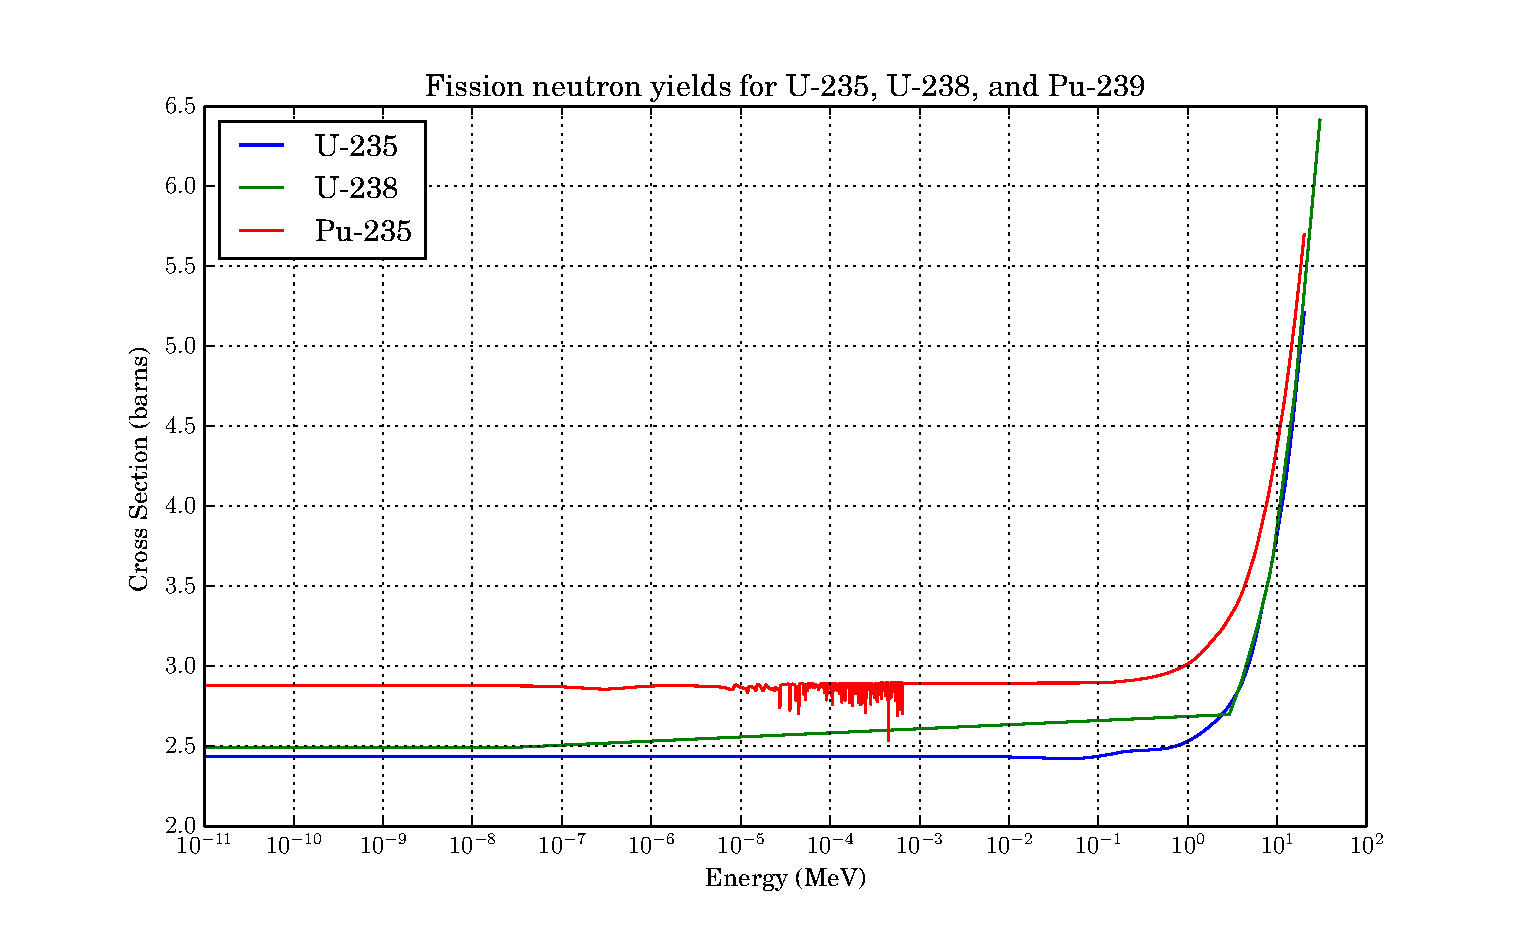
\includegraphics[width=0.8\textwidth]{graphics/nu_compare.eps}
     \caption{Total fission yield, $\nu_\mathrm{T}$, for uranium-235, uranium-238, and plutonium-239.}
\end{figure}

\begin{figure}[h!]
  \label{xs_fission_only}
  \centering
    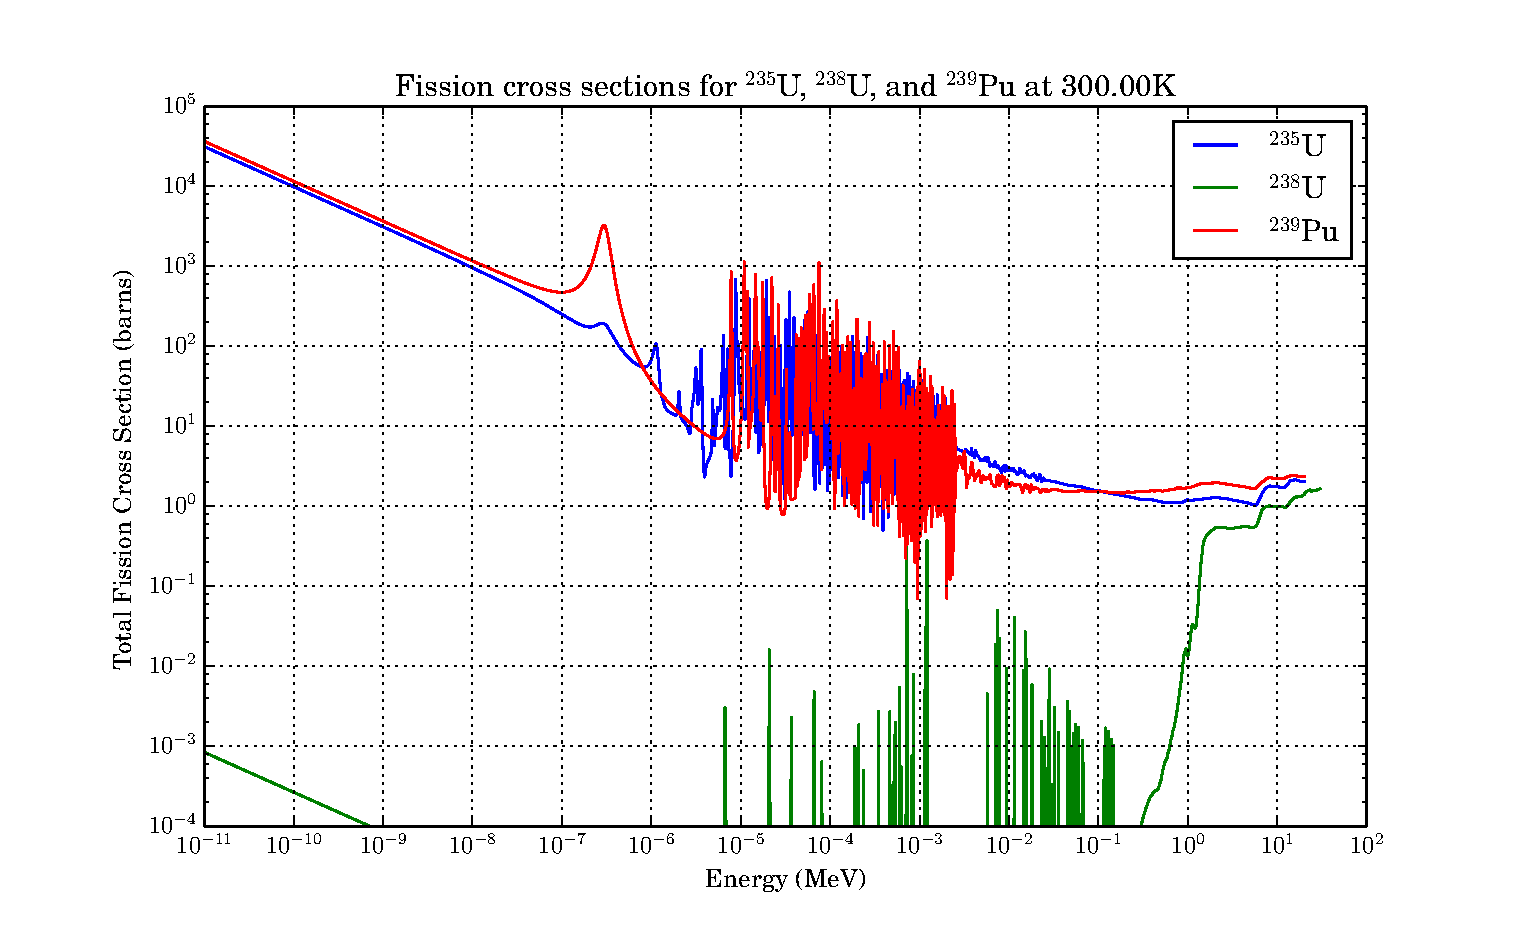
\includegraphics[width=0.8\textwidth]{graphics/xs_fissile.eps}
     \caption{Fission cross sections for uranium-235, uranium-238, and plutonium-239.}
\end{figure}

Figure \ref{nu_compare} shows the energy dependence of the total fission neutron yield, $nu_\mathrm{T}$. It is shown at one temperature since it have very weak temperature dependence.   It can be seen that it is constant until energies in the MeV range, where it increases sharply due to the energy the incident neutron provides being sufficient to eject a bound neutron.  Figure \ref{xs_fission_only} shows the total fission cross sections for two \emph{fissile} isotopes, uranium-235 and plutonium-239, and one \emph{fertile} isotope, uranium-238.  Fissile isotopes are those which neutrons at any energy can induce fission.  The figure shows that uranium-238 has a fission cross section, but it isn't significant until above 1 MeV.  For uranium-238, fission is a threshold reaction.  Simply absorbing a neutron does not provide enough energy to split the nucleus.  Additional energy is required, which can be provided in the form of an incident neutron's kinetic energy.  Uranium-238 isn't fissile, but it can be a significant contributor of fission reactions in reactors where the neutron population is \emph{fast}, i.e. mainly high-energy.  As mentioned before, uranium-238 is considered fertile, which means that it produces a fissile isotope after it absorbs a neutron, and in this case decays to plutonium-239.  

Fission spectrum?

\subsubsection{Other Inelastic Secondary-Producing Reactions}

This category encompasses all the other reactions neutrons undergo.  There are two types, ones that produce secondary neutrons in some amount and those that do not.  Those that do not may still produce other particles, like alpha particles, tritons, protons, et cetera.  Since they do not produce secondary neutrons, however, they are basically equivalent to a disappearance reaction in the scope of neutron transport.  Even though they aren't capture reactions, they can contribute significantly to an isotope's absorption of neutrons.  Figure \ref{xs_e_dependence_li} shows that the (n,$^3$H) in lithium-6 is by far the main component of the total cross section and makes it a very strong absorber of low energy neutrons.  Boron-10 is another great example of this.  Its (n,$\alpha$) reaction has a very high cross section for low energy neutrons, and it is widely used in thermal spectrum reactors in safety and control systems.

Of the reactions that produce secondary neutrons, the (n,2n) reaction is most significant, due to it having the lowest threshold energy.  At higher incident neutron energies, (n,3n) and even (n,4n) can become possible.  Other particle combinations are possible as well, such as (n,n$\alpha$), and these reactions act like an inelastic scatter interaction where the relationship between scattering angle and energy no longer applies due to there being three bodies to distribute energy to instead of only two.

%%%%%%%%%%%%%%%%%%%%%%%%%%%%%%
\subsection{Temperature Effects}

Thus, far there has only been mention of the target nuclide's by how it manifests itself in the 1/$v$ behavior of cross sections at low energy.  Most of the time, it is a good assumption that the thermal motion of the target nuclide is negligible.  Thermal energy is on the order of .01 eV, and this is a good assumption when neutrons are at MeV range energies, but when they scatter and lose energy, they can come near the thermal energy of the material.  When this happens, the target nuclide no longer appears stationary, and assuming that it has zero velocity in scattering calculations is inaccurate.  MCNP sets the threshold at 400kT, which corresponds to about 10 eV for materials at room temperature, above which the target nuclide can be assumed stationary.  Below this threshold, it is important to model thermal effects.  If this wasn't done, a neutron could keep scattering off of zero-energy targets and it's energy could approach zero, which is not physical.  Neutrons can only scatter down to a state where they are in thermal equilibrium with the material they are traveling through.  This creates a ``thermal peak'' at low energies where neutrons collect, especially in materials where the scattering cross section is large and neutrons scatter many times before they are absorbed.

\begin{figure}[h!]
  \label{MB_dist}
  \centering
    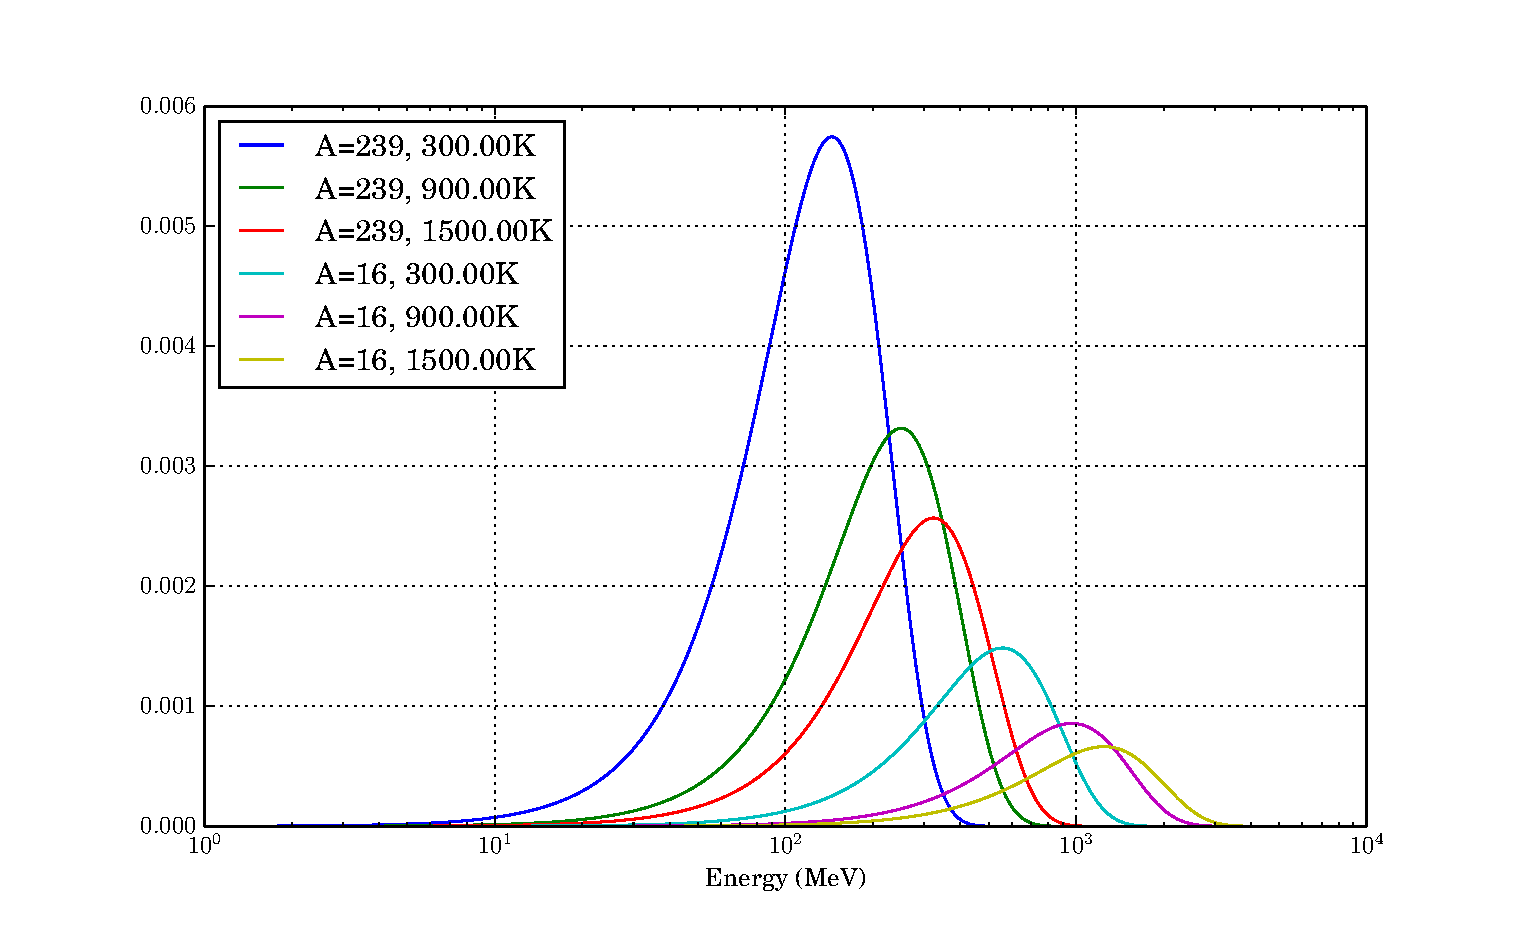
\includegraphics[width=0.8\textwidth]{graphics/MB_dist.eps}
     \caption{Maxwell-Boltzmann distribution for the speed of heavy and light nuclides at different temperatures.}
\end{figure}


\subsubsection{Doppler Effect}


The other effect that thermal motion has is the \emph{Doppler effect}.  This is where resonances are broadened as temperature increases due to the thermal distribution becoming wider.  The effect is also known as \emph{Doppler broadening} for this reason.  Figure \ref{MB_dist} shows the Maxwell-Boltzmann distributions at various temperatures for a heavy particle and for a light particle.  This is the distribution of speeds particles in a ``gas'' have if they only interact by scattering off of one another.  Most solids can be modeled as a dense gas when there are no strong anisotropies in their structure, which is why modeling the target velocities in this way is called the ``free gas model.''  Note that the broadening effect is much more pronounced for light nuclei.  

The widening of resonances effects reactors in significant ways, most notably in that more neutrons are absorbed in the resonance region as the scatter down to thermal energies.  The number of neutrons lost to capture increases and reduces the overall multiplication factor.  It is important for reactor safelt that this occurs since it produces a negative reactivity feedback for temperature and helps prevent power excursions and meltdowns.  If the multiplication factor is above unity, the power starts to rise, and therefore so does the temperature (if the coolant flow rate remains the same).  When the temperature goes up, the increased captures causes it to go back down, stopping the power from increasing.  Of course, there are many different types of reactivity feedback phenomena, but the temperature feedback is generally negative due to Doppler broadening.  Capture is increases most in fission products since they often have strong absorption resonances and are lighter than fuel nuclides.  Very light nuclides typically do not have absorption resonances, so Doppler broadening has littler effect on their absorption rates.  This is why temperature feedback is least effective in fresh fuel where there are few fission products.  Figure \ref{xs_eu_broaden} shows the effect in europium-155, a fission product with a high capture cross section.

\begin{figure}[h!]
  \label{xs_eu_broaden}
  \centering
    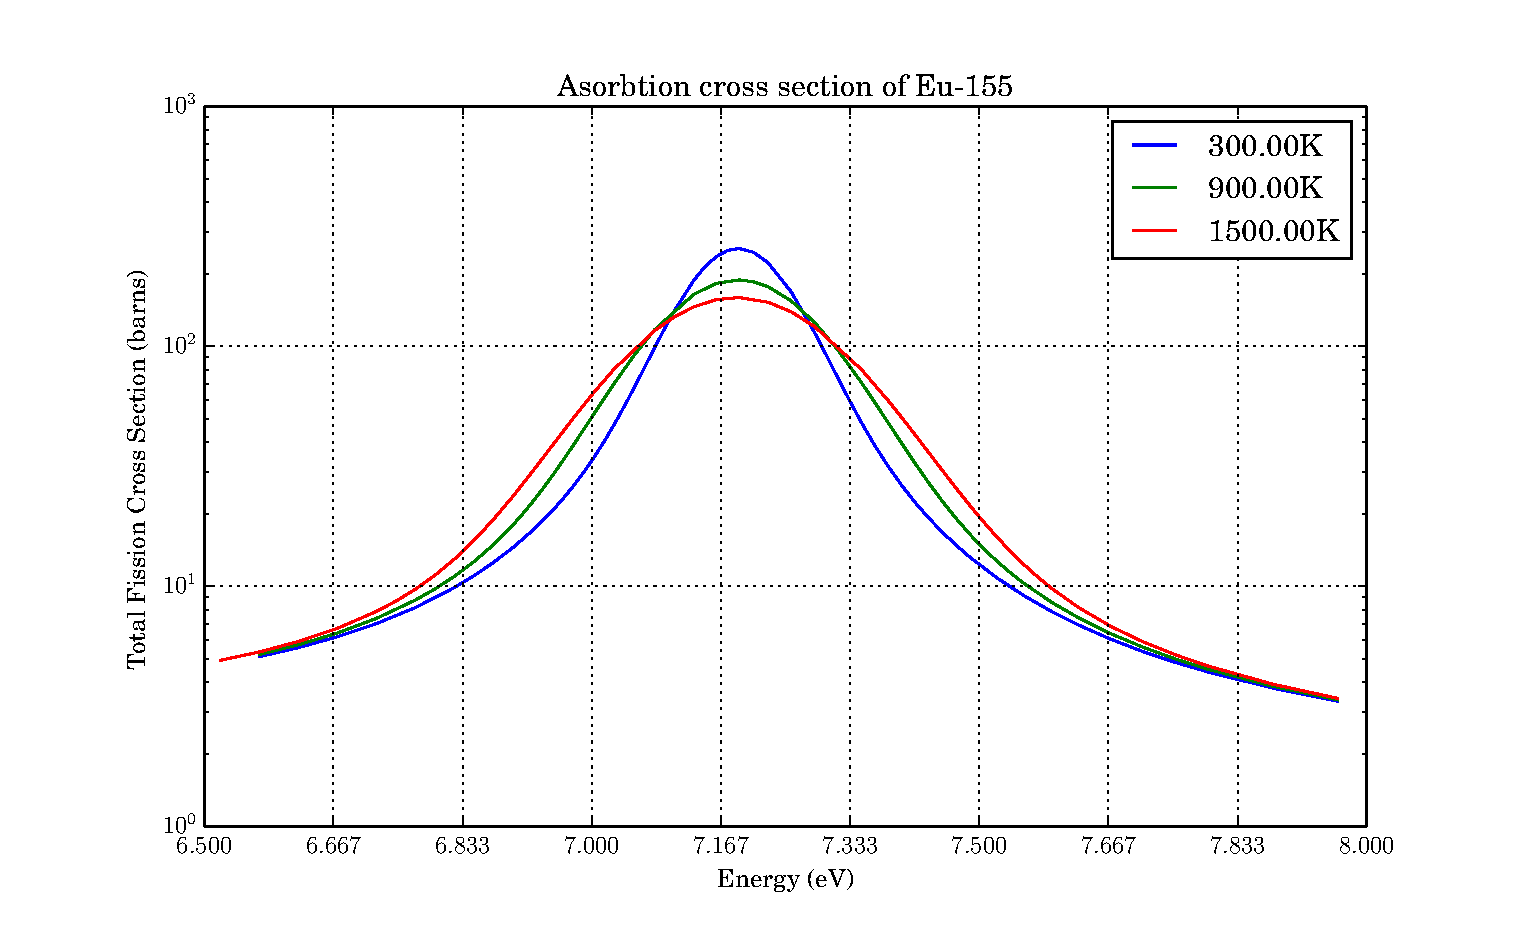
\includegraphics[width=0.8\textwidth]{graphics/xs_eu_broaden.eps}
     \caption{Doppler broadening of the 1eV fission resonance in Eu-155.}
\end{figure}

At 0K, resonances are very sharp and can be treated as delta functions.  To make the assumption that the target is at rest, the thermal distribution must be convolved with the cross section to order to account for the different speeds the targets are moving.  This is especially significant at resonances since slight movements in velocity can produce very large differences in cross section.  The exact method for doing this is shown in \eqref{broaden}\cite{Cullen_Weisbin_1976}.

\begin{equation}
\begin{split}
Find a copy\\
of the paper!
 \end{split}
\label{broaden}
\end{equation}

Then say some things about it once you get details, particularly that it is an expensive operation

%%%%%%%%%%%%%%%%%%%%%%%%%%%%%%
\subsection{Nuclear Data}

Cross section data is distributed by the Department of Energy in \emph{ENDF} files.  ENDF stands for ``evaluated nuclear data file,'' and can contain data for nuclear decay, photons, atomic relaxation, fission yields, thermal neutron scattering, and charged particle reactions as well as neutron reactions.  They are called ``evaluated'' because an organization decides, or evaluates, which experimental data is the highest quality and will be included in the final dataset.  They also decide how to represent regimes that haven't been measured yet by comparing simulation results to experiments.   The first data released was ENDF/B-I in 1968 and the latest set is ENDF/B-VII, which was released in 2006.  They have a standard format that dates back to when the data was stored on magnetic tapes, and are sometimes referred to as ``tapes'' to this day.  The format is rather archaic and contains a lot of redundant information about record locations which was useful when the tape head had to physically move between points in the tape.  

\begin{figure}[h!]
  \label{data_levels}
  \centering
    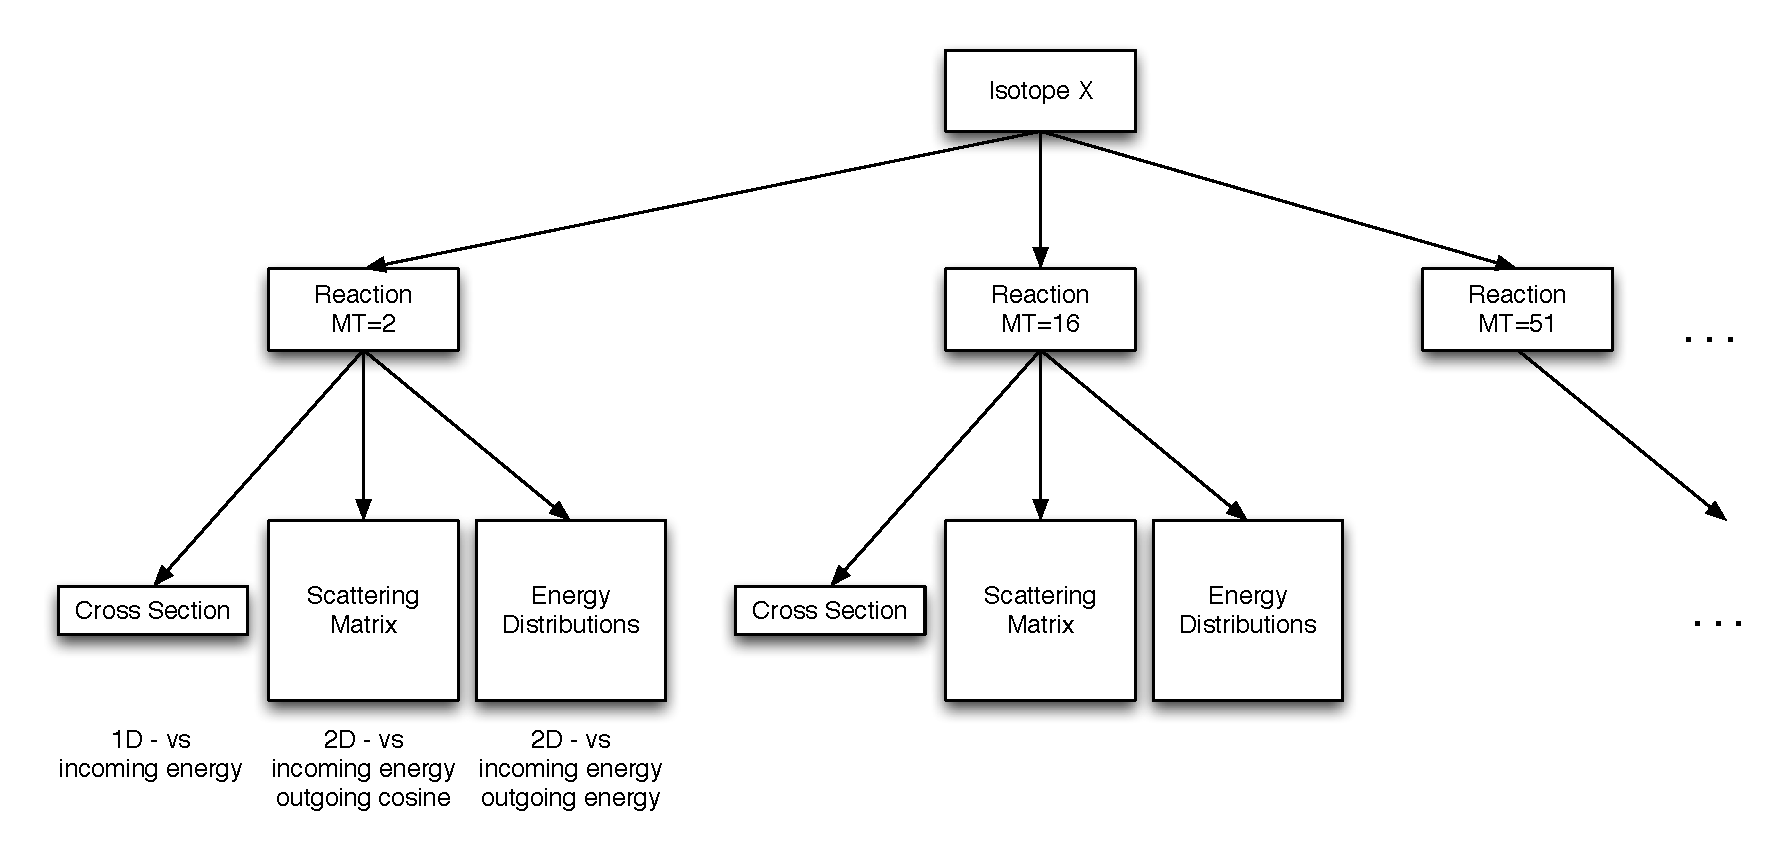
\includegraphics[width=0.8\textwidth]{graphics/data_levels.eps}
     \caption{Hierarchy in ACE formatted neutron data libraries.}
\end{figure}

Many Monte Carlo codes read ACE formatted data rather than the original ENDF file.  ACE stands for ``a compact ENDF'' and strips out a lot of the extra information unnecessary for neutron transport.  As Figure \ref{data_levels} shows, ACE files not only contain cross sections, but also angle and energy distributions used in scattering and fission.  ENDF assigns a number to each type of reaction called the \emph{MT} number.  Table \ref{MT_numbers}, taken from a LANL website, shows the major numbers \cite{MTnums}.  It can clearly be seen that there are many reactions a neutron can undergo, most of which have very energy strong dependance.  Most of the complexity in modeling nuclear reactors comes from the fact that the data needed to model neutrons is very complicated.  It may be the most important part of the simulation, it is what ties the calculations to reality.  If inaccurate data is used, the results will not have any physical meaning, and the simulation becomes a mathematical exercise. 

%%%%%%%%%%%%%%%%%%%%%%%%%%%%%%
\subsection{Neutron Transport}

Now that the events which can happen to neutrons have been outlined, we will move to describing the neutron population itself.  Since the neutron population in reactors is large, on the order of $10^{XXX}/\mathrm{cm}^3$, and the neutrons themselves have very small radii, about $1.75\times10^{-17}$ cm, the distribution of neutrons can be treated as an continuum.  We will eventually derive the \emph{neutron transport equation}, which is a linearized version of the Boltzmann transport equation.  It is linear since it is assumed that neutrons do not interact with each other.  This is usually a good assumption in normal matter since the neutron density present in reactors is many orders of magnitude smaller than the material density and neutrons are much more likely to interact with it than each other.  

Other than eliminating neutron self interaction, there are a handful of other assumptions that go into the equation that will hold true for the rest of the derivations.  One that follows veery closely is that neutrons are assumed to be points in space, so even at very high densities they sill will not interact with each other, and later when we start to discretize spaces, neutrons cannot be in more than one unique volume by overlapping.  The next assumption is that any relativistic effects are negligible.  The energies of importance in reactor physics are below 10MeV, which is about where they start to become non-negligible for neutrons.  Since neutrons are neutral and have long interaction distances compared to their radii, they are also assumed to move in straight lines between collisions.  Materials are also assumed to be in thermal equilibrium and have isotropic properties.  Materials like graphic and water do not have isotropic properties when it comes to scattering, however.  As will be explained later, this can be corrected by adjusting the scattering kernel.

\subsubsection{Neutron Balance Equation}

\begin{figure}[h!] 
  \label{diff_volume}
  \centering
    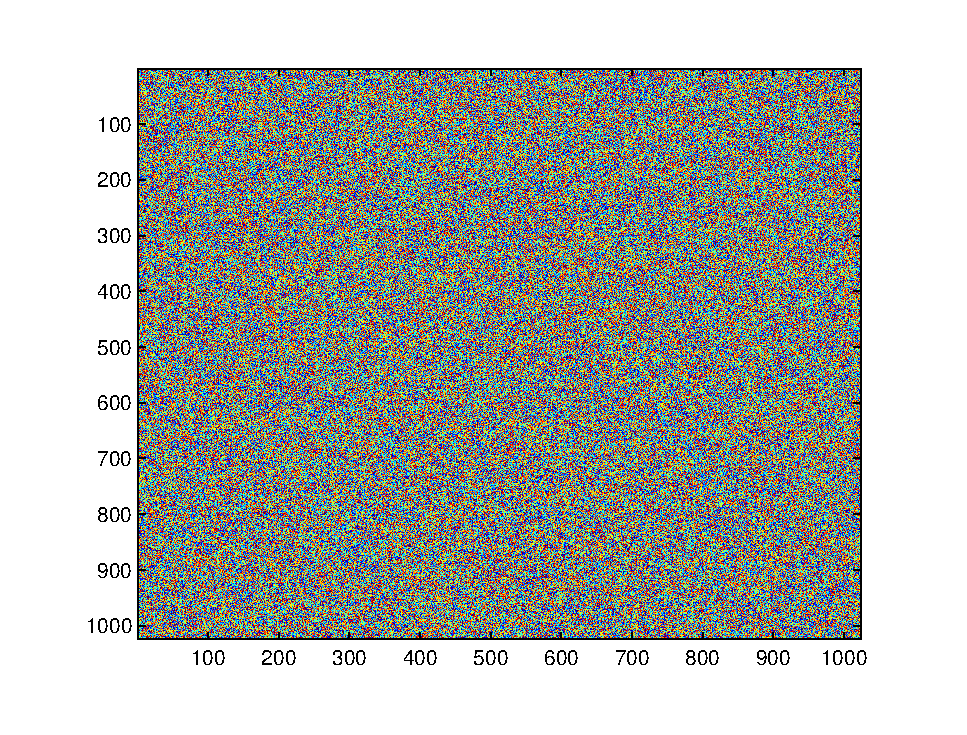
\includegraphics[width=0.8\textwidth]{graphics/noise.eps} 
     \caption{The differential volume of the neutron balance equation.}
\end{figure}

Before any explicit terms need to defined to capture the necessary physics of the transport problem, a balance equation can be written for a differential volume.  This equation simply describes the amount of neutrons entering and exiting a infinitesimally small volume and their difference being equal to the rate of change of neutrons in the volume.  We know about the reactions that neutrons can undergo, and we know they move through material, so we should have  enough information the write this abstract equation. Figure \ref{diff_volume} shows an illustration of the differential volume.

\begin{equation}
\footnotesize
\label{NBE}
\begin{array}{c}
\mathrm{rate\:of\:change} = (\mathrm{neutrons\:in}) - (\mathrm{neutrons\:out}) \\
\\
\frac{\partial n}{\partial t} = ( \mathrm{movement\:in} + \mathrm{source} + \mathrm{scatter\:in}) - ( \mathrm{movement\:out} + \mathrm{disappearance} + \mathrm{scatter\:out})
\end{array}
\end{equation}

Now that this equation has been written, we can start to explicitly define the terms.  One quantity has already been touched upon - the neutron density.  The neutron density is the fundamental quantity in reactor physics.  This is shown in \eqref{NBE} as $n$, but in the subsequent sections its dependencies will be elaborated on, as will all other dependencies.


\subsubsection{Neutron Distribution Function}

The \emph{neutron distribution function} simply describes the number of neutrons present in each differential quantity it represents.  The most detailed version is differential in space, angle, energy (or velocity), and time, and has inverse units of these dimensions.  In other words, it describes a density in each of it components.  In the subsequent derivations, the spatial, or position vector will be represented by $\boldsymbol{\vec{r}}$, the angular vector by $\boldsymbol{\hat{\Omega}}$, energy by $E$, and time by $t$.  The angle vector is a unit vector that specifies direction only, not magnitude.  It is easiest to express the directional vector as a unit vector in spherical coordinates $(\theta, \phi)$, the polar angle and the azimuthal angle, respectively.  Their cartesian projections are given by \eqref{ang_cart} and shown in Figure \ref{ang_relations}.

\begin{equation}
\label{ang_cart}
\begin{split}
\Omega_x &= \sin \theta \sin \phi  \\
\Omega_y &= \sin \theta \cos \phi \\
\Omega_z &= \cos \theta = \mu
\end{split}
\end{equation}

\begin{figure}[h!] 
  \label{ang_relations}
  \centering
    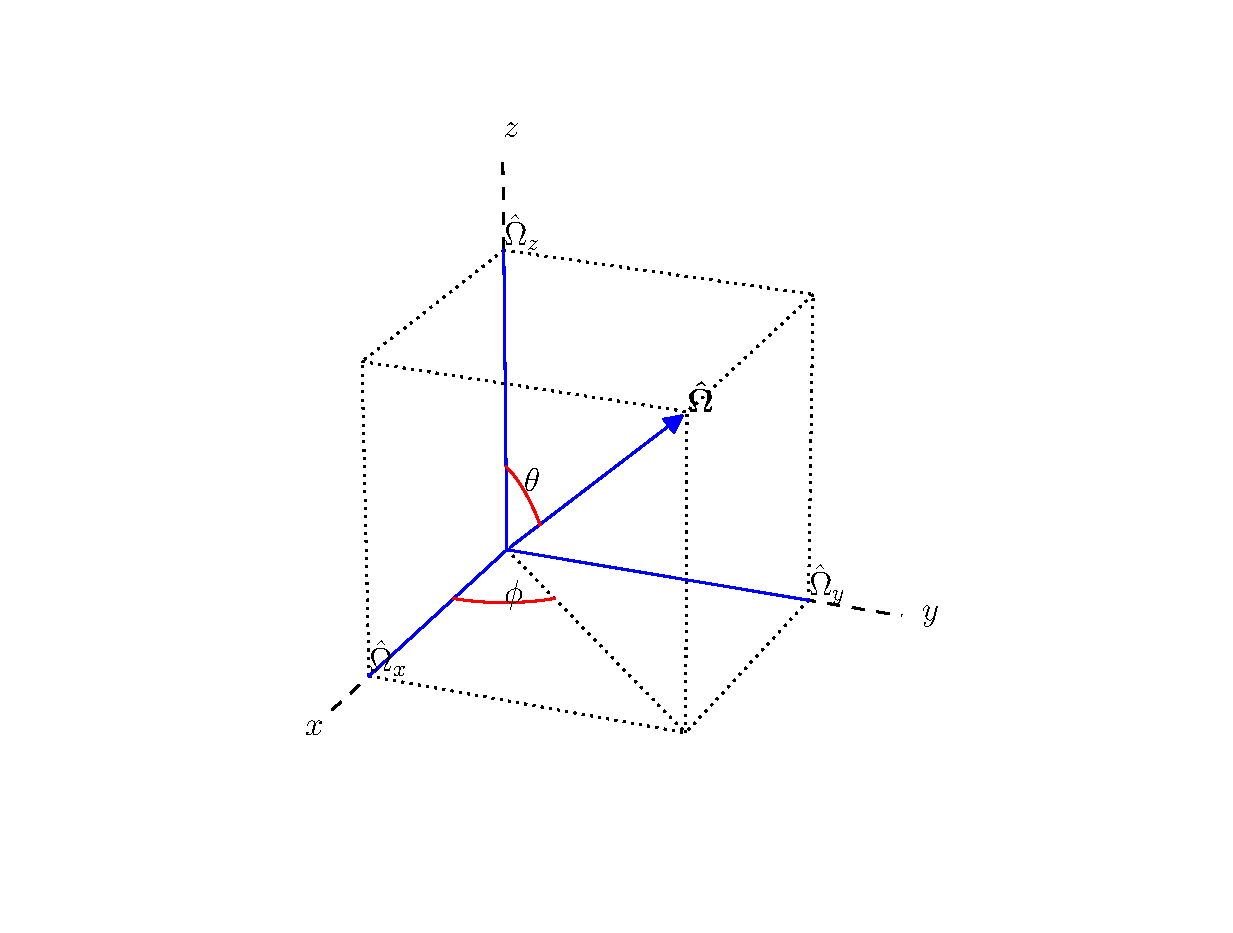
\includegraphics[width=0.8\textwidth , trim= 0cm 2.5cm 0cm 0cm]{graphics/ang_relation.eps} % trim = l b r t
     \caption{The cartesian projections of the directional vector.}
\end{figure}

Like any continuous distribution, it must be integrated over to calculate any quantities.  If we define the $i$th moment of the distribution according to \eqref{NDF_moments}, then the $0$th moment would be the population and the $1$st moment would be the mean.

\begin{equation}
\label{NDF_moments}
M_i = \int_{-\infty}^{\infty} n(x)  x^{i} dx
\end{equation}

For example, if we are given a neutron distribution which has no time dependence, $n(\boldsymbol{\vec{r}},\boldsymbol{\hat{\Omega}},E)$, and wanted to calculate the total number of neutrons present in a volume V, we would calculate this number by \eqref{NDF_sample}, whereas if we wanted to know the average energy, we would do this by \eqref{NDF_avg}.

\begin{equation}
\label{NDF_sample}
N_V = \int_0^\infty \int_{\boldsymbol{\hat{\Omega}}} \int_{V} n(\boldsymbol{\vec{r}},\boldsymbol{\hat{\Omega}},E) dV d\boldsymbol{\hat{\Omega}} dE
\end{equation}

\begin{equation}
\label{NDF_avg}
\bar{E} = \int_0^\infty \int_{\boldsymbol{\hat{\Omega}}} \int_{V} E n(\boldsymbol{\vec{r}},\boldsymbol{\hat{\Omega}},E) dV d\boldsymbol{\hat{\Omega}} dE
\end{equation}

\subsubsection{Reaction Rates}

A \emph{reaction rate} is the rate at which a certain reaction is happening in a volume.  If we go to a pulse-type scenario once more, we have $N_\mathrm{p}$ particles which travel at speed $v$ in one direction.  If $\Sigma$ is the interaction probability per unit length, multiplying it by the speed gives the probability of interaction per second, or the \emph{collision rate}.  Since there are $N$ particles, multiplying the rate by it gives the overall reaction rate, $N_\mathrm{p} v \Sigma$, of the pulse in an infinite medium.  If $N$ is now substituted for the neutron distribution function instead of a pulse, the expression now becomes the reaction rate per distribution differential, or the \emph{reaction rate density}.  This expression is shown in \eqref{RR} and is the first building block of the \emph{neutron balance equation}.

\begin{equation}
\label{RR}
R(\boldsymbol{\vec{r}},\boldsymbol{\hat{\Omega}},E,t)  = v(E) n(\boldsymbol{\vec{r}},\boldsymbol{\hat{\Omega}},E,t) \Sigma(\boldsymbol{\vec{r}},E)
\end{equation}

If we assume there is only one energy, $E_0$ and one direction, $\hat{x}$, and integrate over the constant dimensions of this equation, as shown in \eqref{1d_diff}, we get an expression for the reaction rate in an infinitesimal slice dx.  $A$ is the area perpendicular to the direction of motion where the neutron population is nonzero.


\begin{equation}
\label{1d_diff}
\int_A \int_{\boldsymbol{\hat{\Omega}}} \int_0^{\infty}  dE d\boldsymbol{\hat{\Omega}} dxdydz  v(E) n(\boldsymbol{\vec{r}},\boldsymbol{\hat{\Omega}},E,t) \Sigma(\boldsymbol{\vec{r}},E) \delta(E-E_0) \delta(\boldsymbol{\hat{\Omega}}-\hat{x})  = v \Sigma A n(x)dx 
\end{equation}

This is effectively the loss term for a beam in the $\hat{x}$ direction, and if we set it as such, we recover the beam-type expression \eqref{recover_beam}, which is equivalent to \eqref{pop_diff}.  

\begin{equation}
\label{recover_beam}
dn(x) = - v \Sigma A n(x)dx  \qquad \Rightarrow \qquad  \frac{dI(x)}{dx}= - \Sigma I
\end{equation}



\subsubsection{Angular and Scalar Flux}

Since the reactions rate density is dependent on the cross section and the velocity multiplied by the neutron distribution, this quantity is redefined as the \emph{angular flux} as shown in \eqref{ang_flux}.  Flux meaning that it represents a rate at which particles are passing through a surface, and angular meaning that it is differential in angle.  Again, since the reactions rates depend on this quantity, the neutron transport problem is usually written in terms of the angular flux, which is then solved for instead of the neutron distribution.

\begin{equation}
\label{ang_flux}
\psi(\boldsymbol{\vec{r}},\boldsymbol{\hat{\Omega}},E,t) = v(E) n(\boldsymbol{\vec{r}},\boldsymbol{\hat{\Omega}},E,t)
\end{equation}

Scattering and neutron movement have angular dependence, but reaction cross sections do not, so the reactions can be written in terms of angular flux which has been integrated over all angles, or the \emph{scalar flux} or simply the \emph{flux}.  The relation between the two fluxes is show in \eqref{scalar_flux}.  This is usually the most interesting quantity in reactor physics since the reactor power profile is directly proportional to it.  The reaction rate for a reaction $i$ is shown in \eqref{scalar_flux_RR}.

\begin{equation}
\label{scalar_flux}
\phi(\boldsymbol{\vec{r}},E,t) = \int_{4\pi} \psi(\boldsymbol{\vec{r}},\boldsymbol{\hat{\Omega}},E,t)
\end{equation}

\begin{equation}
\label{scalar_flux_RR}
 R_i(\boldsymbol{\vec{r}},E,t) = \int_{4\pi} \Sigma_i(\boldsymbol{\vec{r}},E) \psi(\boldsymbol{\vec{r}},\boldsymbol{\hat{\Omega}},E,t) = \Sigma(\boldsymbol{\vec{r}},E) \int_{\boldsymbol{\Omega}} \psi(\boldsymbol{\vec{r}},\boldsymbol{\hat{\Omega}},E,t) = \Sigma(\boldsymbol{\vec{r}},E) \phi(\boldsymbol{\vec{r}},E,t)
 \end{equation}

\subsubsection{Scattering}

Scattering is highly dependent on angle and energy and requires as more detailed cross section than disappearance reactions.  Elastic scattering has a fixed relation between outgoing energy and angle, but inelastic scattering does not.  Scattering moves a neutrons energy and angle, so to be completely general in describing it, the cross section is assumed to not only ne dependent on incoming energy like all other cross sections, but also on outgoing energy, incoming angle, and outgoing angle.  Since two quantities are being related before and after a scattering event, the scattering cross section is considered \emph{doubly differential} and is sometimes called the \emph{scattering kernel} whereas the integrated value which only depends on incoming energy is called the scattering cross section.   An expression for the scattering kernel is shown in \eqref{scattering_DD_xs} with the incoming values primed.

\begin{equation}
\label{scattering_DD_xs}
\Sigma_s = \Sigma_s(E^\prime \rightarrow E,\boldsymbol{\hat{\Omega}}^\prime \rightarrow \boldsymbol{\hat{\Omega}})
 \end{equation}

There is a practical reason for separating scattering into a total cross section that describes its likelihood, or probability of a neutron entering the reaction, and a kernel that describes how it exits.  In a Monte Carlo simulation, the cross section is used to determine \emph{whether} scattering happens rather than \emph{how} it happens.  The scattering kernel is only used if a neutron has already been determined to scatter.  This is also shown in the expressions for the scattering in a differential volume.  The cross section is used as the removal of a neutron from a particular energy, whereas the kernel is used to determine from which other energies and angles a neutron is scatter \emph{into}.  This can be seen in \eqref{scattering_DD_xs}.  If the outgoing energy and angle are held constant, the quantity is the probability which other angles and energies scatter into it.

Using these two quantities, source and loss terms can be written for scattering.  The expression for loss uses the cross section, shown in \eqref{scattering_loss}, and the kernel is used in what is often called the \emph{scattering source} term, shown in \eqref{scattering_source}.  The source term need to be integrated over all other energies $E^\prime$ and angles, $\boldsymbol{\hat{\Omega}}^\prime$, which neutrons can scatter into energy $E$ and angle $\boldsymbol{\hat{\Omega}}$.

\begin{equation}
\label{scattering_loss}
R_{s, \mathrm{loss}}( \boldsymbol{\vec{r}},\boldsymbol{\hat{\Omega}},E,t ) = \Sigma_s (\boldsymbol{\vec{r}},E) \psi(\boldsymbol{\vec{r}},\boldsymbol{\hat{\Omega}},E,t)
 \end{equation}
 
 \begin{equation}
\label{scattering_source}
R_{s, \mathrm{source}}(\boldsymbol{\vec{r}},\boldsymbol{\hat{\Omega}},E,t) = \int_0^\infty  \int_{4\pi} \Sigma_s(E^\prime \rightarrow E,\boldsymbol{\hat{\Omega}}^\prime \rightarrow \boldsymbol{\hat{\Omega}}) \psi(\boldsymbol{\vec{r}},\boldsymbol{\hat{\Omega}}^\prime,E^\prime,t) d\boldsymbol{\hat{\Omega}}^\prime dE^\prime
 \end{equation}
 

\subsubsection{Streaming}

So far all that has been  touched on is how neutrons within a volume move in angle and energy or are removed outright.  Now we will go over how they move in space, and to do this we consider a surface $S$ around our differential volume.  We want to find an expression for the net number of neutrons passing through this surface and this will be our net leakage term (incoming minus outgoing).  The angular neutron flux describes the number of neutrons crossing a differential surface at angle $\boldsymbol{\hat{\Omega}}$, but in order to perform any vector operations on it, we must multiply it by the unit vector.  We can then write and expression for the leakage by performing a surface integral over the current and surface normal's dot product, shown in \eqref{leakage_surface}.

\begin{equation}
\label{leakage_surface}
\mathrm{Leakage} = \int_S ds \cdot \boldsymbol{\hat{\Omega}} \psi(\boldsymbol{\vec{r}},\boldsymbol{\hat{\Omega}},E,t)
\end{equation}
 
 We can turn this into a volume integral by applying the divergence theorem, shown in \eqref{div_theorem}.  If the volume of interest is shrunk to an infinitesimal volume and we switch the order of the dot product, we come to an expression that can be used in the balance equation.  This expression, shown in \eqref{streaming}, is often called the \emph{streaming} term, since it describes the net movement of neutrons into the differential volume due to their physical movement.
 
\begin{equation}
\label{div_theorem}
\int_S ds \cdot \boldsymbol{\hat{\Omega}} \psi(\boldsymbol{\vec{r}},\boldsymbol{\hat{\Omega}},E,t) = \int_V dV \nabla \cdot \boldsymbol{\hat{\Omega}}  \psi(\boldsymbol{\vec{r}},\boldsymbol{\hat{\Omega}},E,t)
\end{equation}

\begin{equation}
\label{leakage_surface}
 \lim_{V\to dV} \int_V dV \nabla \cdot \boldsymbol{\hat{\Omega}}  \psi(\boldsymbol{\vec{r}},\boldsymbol{\hat{\Omega}},E,t) =  \boldsymbol{\hat{\Omega}}  \cdot \nabla\psi(\boldsymbol{\vec{r}},\boldsymbol{\hat{\Omega}},E,t) 
 \end{equation}


\subsubsection{Neutron Transport Equation}

Now we have al terms we need to write down a full transport equation

\section{Discrete Methods}

moments

Diffusion, SN

drawbacks, limitations

\section{Monte Carlo}

instead of the neutron population being continuous and the spatial and energy dimensions discretized (and integrating along them), we make the population discrete (and integrate over it) and leave the other dimensions continuous! 

equations and derivations and such

advantages, parallel scaling, low assumptions, high fidelity geom

drawbacks and limitations

\subsection{Sampling Schemes}

\subsubsection{Interpolation}

``Continuous Energy'' = interpolation

\subsubsection{Distance To Collision}
Macro


\subsubsection{Reaction Type}
micro

\subsubsection{Free Gas Treatment}


\subsubsection{Elastic Scattering}


\subsubsection{Inelastic Reactions}


\subsubsection{Fission}

fission dist

source pop



%%%%%%%%%%%%%%%%%%%%%%%%%%%%%%

\section{GPUs}

Part of the reason GPUs are able to perform efficiently is do to their reliance on single instruction, multiple data (SIMD) execution.  This execution method uses the same instructions carried out over multiple pieces of data at the same time.  This reduces the amount of power used in control and therefore more math can be done per watt [citation definitely needed].  The GPU programming model abstracts SIMD execution by using threads, which can be thought of in the traditional sense . There are some tradeoffs, however, including limited on-board memory (currently 12 GB), limited cache and control space, and requiring data parallelism for full utilization.

Since all threads in a GPU thread block must execute the same instructions, having conditional statements based on random numbers can cause threads to be serialized, leading to resource under-utilization.  For example, in particle transport where a particle history is assigned to each thread, thread divergence mainly arises through particles undergoing different reactions based on the results of cross-section sampling.  Also, GPUs have even higher global memory latency than CPUs, up to 800 clock cycles on older cards, compared to about 50 cycles on a typical CPU.  It is also important to remember than GPUs are clocked much slower than CPUs, so the memory latency performance issue is even greater [5, 7]. 

another brief introduction.  

advantages

pitfalls, weaknesses

\subsection{Supercomputing}

how and why they came to be used for supercomputing.

\subsection{Architecture}

SIMD, threads

\subsection{Memory}

speed, levels, etc.  limitations 

\subsection{CUDA}

kernels

%%%%%%%%%%%%%%%%%%%%%%%%%%%%%%

\section{Previous Works}

talk about the work that other people did

\section{Preliminary Studies}

all my prelim work to motivate this project

\subsection{2D Scattering Game}


\subsection{Ray Tracing with OptiX}

%%%%%%%%%%%%%%%%%%%%%%%%%%%%%%

\section{Scope in Detail}


